\chapter{Theorie der Pathfinding-Algorithmen}

\section{Grundwissen}

\subsection{Was sind Algorithmen}

Ein Algorithmus beschreibt eine abstrakte Form eines Aufgabenlösungswegs.
Er besteht aus klaren Handlungsvorschriften, die in Form einer Kette
oder Reihe in Einzelschritten abgearbeitet werden, um ein Problem
zu lösen. Ein Algorithmus kann den Satzaufbau einer Sprache
vorschreiben (Subjekt, Verb, Objekt) oder die Herstellung eines Gerichts
in der Küche als Kochrezept. Es wird immer eine bestimmte Eingabe in
eine bestimmte Ausgabe verarbeitet. Das Ergebnis ist dabei immer das
Gleiche, ähnlich wie bei einer Funktion in der Mathematik.

Es gibt sehr einfache Algorithmen, wie Verhaltensregeln oder Gesetze, in
denen man nachschauen kann, wie man sich in welcher Situation verhält
oder was erlaubt ist. Schwierigere Algorithmen findet man eher in der
Mathematik, Datenanalyse oder auch im Bewusstsein der Menschen.
\cite[Wikipedia, 2018]{wikialgo}

\subsection{Was ist ein Pathfinding-Algorithmus}

Die Pathfinding-Algorithmen sind eine Unterklasse der Algorithmen, sie
spezialisieren sich auf die suche des optimalsten Wegs von einem Punkt $A$
zu einem anderen Punkt $B$ in einem Raum. Der Raum oder die Matrix kann hierbei
zweidimensional oder dreidimensional sein, in dieser Arbeit befassen wir
uns nur mit den Pathfinding-Algorithmen im zweidimensionalen Raum.

Bei Computerspielen kann der Raum das Spielfeld sein, wo unter anderem
eine Computergesteuerte Person (künstliche Intelligenz $=$ KI) immer auf
den Spieler zuläuft oder ihn in einem definierten Abstand umkreist.

Bei der heutigen Internetinfrastruktur helfen Pathfinding-Algorithmen unsere Daten über Routenplanung effizient von unserem
Computer zum Server der aufgerufenen Website zu leiten und wieder zurück.

Die Pathfinding-Algorithmen suchen sich generell den kostengünstigsten
oder kürzesten Weg mit wenig Hindernissen aus. Ein Vogel kann mühelos
über einen Berg fliegen und legt bloss die direkte Luftlinie als
Wegstrecke zurück, wir Menschen müssen meistens um den Berg herum reisen
oder ihn in schlangenlinigförmigen Wanderwegen überwinden.

Ob dieser Wanderweg der optimalste ist, hängt von verschiedenen Faktoren
ab, da es eventuell sinnvollere Wege zum Ziel gibt.

\begin{itemize}
\item
  \textbf{Zeitoptimierung}: Man möchte am schnellsten am Ziel sein, vorzugsweise sucht man sich
  eine öffentliche Fortbewegung wie ein Bus.
\item
  \textbf{Kostenoptimierung}: Man hat nicht unbegrenzt Geld und sucht sich den kostengünstigsten Weg
  heraus.
\item
  \textbf{Wegoptimierung}: Man möchte auf der Wanderung von gewissen Orten Bilder mit der Kamera
  festhalten.
\end{itemize}

Man beachte, dass egal welcher Weg ausgewählt wurde, dieser immer Vor-
und Nachteile aufweist. Dies kann man sich unter einem Kuchendiagramm vorstellen.
Es gibt drei Stücke: Zeitoptimierung, Kostenoptimierung und
Wegoptimierung. Egal für welches Stück bevorzugend man den Kuchen
unterteilt, die anderen werden darunter ``leiden''.
\cite[Wikipedia, 2018]{wikipath}

\section{Einführung der Graphen}

Pathfinding-Algorithmus ``sehen'' keine Wände oder Start- und
Endpunkte. Sie verarbeiten lediglich eingegebene Daten in ausgehende
Daten (Input und Output). In unserer Webapplikation vereinfachen die
Pathfinding-Algorithmen die Darstellung des Raumes in nicht-negative
 Graphen (siehe \autoref{chap:nicht-negativ-gewichtet}). Daraus kann abgeleitet
werden, dass die Pathfinding Algorithmen komplett unabhängig von der
visuellen Darstellung des Raumes arbeiten.
\cite[Andreas Hofmann, 2013]{pfbsc}

\subsection{Was ist ein Graph: Graphentheorie und Pathfinder}

Ein Graph ist eine mathematische Struktur zur Darstellung abstrakter
Beziehungsstrukturen und besteht aus zwei Elementen: Ecken/Knoten (engl.
vertices) und Kanten (englisch edges). Jede Kante verbindet exakt zwei
Ecken, es können aber mehrere Kanten auf eine Ecke verweisen. Jeder
angeschaute Knoten vom Algorithmus muss über mindesten eine Verbindung
erreichbar sein.

\begin{figure}[H]
  \centering
  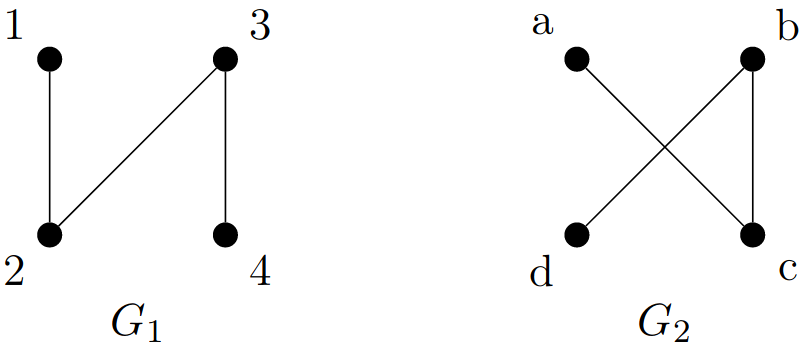
\includegraphics[width=6cm]{graph1.png}
  \caption[Zwei einfache Graphen $G_1$ und $G_2$ mit Ecken und Kanten. Quelle: Benny Sudakov, \textit{Graph Theory}, 2016, ETH Zürich.]{Zwei einfache Graphen $G_1$ und $G_2$ mit Ecken und Kanten. Quelle: Benny Sudakov, \textit{Graph Theory}, 2016, ETH Zürich.}
  \label{fig:graph1}
\end{figure}

Die Knoten stellen bei unserer Anwendung die $x$- und $y$-Koordinaten des Raums
dar und die Kanten die Verbindungen der einzelnen Felder. Somit hat ein
Knoten bei Ausführung des bestimmten Algorithmus 4 Kanten. Wenn dem
Pathfinder die Diagonale zugelassen werden, gelten für die Knoten 8
Kanten.
\cite[Franz Embacher, 2003]{uniwiengraphen}

\subsection{Nicht negativ gewichtet}
\label{chap:nicht-negativ-gewichtet}

In der allgemeinen Graphentheorie sind negativ gewichtete Graphen
erlaubt. Bei den Pathfindern jedoch nicht, da es keine negativen
Distanzen gibt. Von Punkt $A$ nach $B$ gilt eine positive Gewichtung der
Strecke und der Rückweg von $B$ nach $A$ ebenfalls eine positive Gewichtung
der Strecke in den Knoten.
\cite[Krumke; Noltemeier; Schwarz; Wirth, 2000, S. 76]{graphtheoryconcepts}

\subsection{Pathfinding-Graphen}

In unserem Raster kann man sich die Graphenstruktur wie ein Schachbrett
vorstellen. Es beginnt am Startpunkt und sucht Graph um Graph nach dem Ziel.
In jedem Graph wird gespeichert von wo und wessen Nachbargraph man kam und
wie weit man vom Startpunkt entfernt ist. Findet man den gleichen Graph
ein zweites mal, durch einen anderen Weg, wird der schnellere Weg zum
start in den Graph geschrieben. Findet die Struktur das Ziel, so
verweist jeder Vorgehende Graph auf den Graph davor. Diese Graphenkette zeigt dann vom Ziel zum Start.
\cite[Vinther, Vinther, 2015, S. 22]{pftwodim}

%4.3 \#\#\#genauer nachkontrollieren\#\#\#\#\#\#

\section{Heuristiken}

Im Allgemeinen können Algorithmen auf eine Heuristik zugreifen, um
optimierter nach einem Weg zu suchen. Der Begriff ``Heuristik'' bedeutet
mit begrenztem Wissen oder unvollständiger Informationen die optimale
Lösung im Vorhinein zu schätzen. Anders gesagt teilt die Heuristik dem
Algorithmus mit, welcher Graphen am wahrscheinlichsten zum Zielpunkt führt.

Bei den ausgewählten Pathfinding-Algorithmen beim Vergleich benutzt der A* und
BestFirstFinder die Manhattan Heuristik und der BreadthFirstFinder
keine. Der BreadthFirstFinder benutzt in seiner Standardkonfiguration nie eine
Heuristik. Die Manhattan Heuristik, auch Cityblock-Metrik, wurde
ausgewählt, da das Raster dieser Berufsmaturitätsarbeit einem Schachbrett
ähnelt, mit immer dem gleichen Abstand zwischen den Feldern.\\
Die Manhattan-Heuristik wird folgend für alle Punkte im Raster definiert:
\begin{equation*}
d\big((x_1,y_1),(x_2,y_2)\big) = |x_1 - x_{2}| + |y_{1} - y_{2}|
\end{equation*}
Die Distanz $d$ ist gleich der Länge aller Wege, die $P_1$ und $P_2$ entlang der horizontalen und vertikaler Linie verbindet. $P_2$ ist bei dieser Arbeit immer der Zielpunkt und $P_1$ der
aktuelle Standpunkt im Raster. \cite[Patel, 2019]{heuristicsredblob}

\section{Auswahl der Pathfinding-Algorithmen}

Das Autorenteam dieser Arbeit hat sich für folgende Pathfinding-Algorithmen
entschieden, da diese im Vorfeld schon ersichtlich unterschiedliche
Wege im gleichen vorgegebenen Raster ergeben haben.

\subsection{A*}

Der A*-Algorithmus, gesprochen ``A Star'', untersucht mithilfe einer
Heuristik immer den wahrscheinlich nächsten Knoten im Raster, der zum
Ziel führt. Jedem Nachbarknoten wird zuerst einen Wert $d$ zugeordnet, der
angibt, wie lange der Weg geschätzt von diesem Knoten zum Ziel führt. Der Wert $d$
wird mit der Manhattan-Heuristik ausgerechnet. Jeder Graph mit einem $d$-Wert 
wird in eine Liste eingetragen. Der A-Star rechnet immer die neuen
Nachbaren des Graphen mit dem kleinsten $d$-Wert aus. Dadurch kann es
vorkommen, das nach langer Suche der A-Star plötzlich wieder einige
Graphen zurückspringen muss, da die neu berechneten $d$-Werte grösser als
ein früherer gefundener $d$-Wert ist.
\cite[Schmidt, Fuchs]{asterngeo}

\subsubsection{Funktionsweise}

Alle Graphen werden in drei Listen eingetragen:

\begin{itemize}
\item Unbekannte Knoten
\end{itemize}

Bei Starten der Suche sind alle Knoten im Raster in dieser Liste.

\begin{itemize}
\item Bekannte Knoten
\end{itemize}

\begin{quote}
Wurde einem Knoten den d Wert der Heuristik zugeteilt, wird er in diese
Liste mit dem d Wert eingetragen. Aus dieser Liste wird immer der Knoten
mit kleinstem d Wert ausgewählt, der als nächstes angeschaut wird.
\end{quote}

\begin{itemize}
\item Untersuchte Knoten
\end{itemize}

\begin{quote}
Zu diesem Knoten wurde der kleinste Weg herausgefunden, d.h. alle
Nachbarknoten sind in der Liste mit bekannten Knoten.
\end{quote}

Jeder der Gefundenen Knoten besitzt einen Verweis auf den
Vorgängerknoten. Wird das Ziel erreicht, kann mit hilfe dieses Zeigers
der Pfad bis zum Start ausgegeben werden.
\cite[Schmidt, Fuchs]{asterngeo}

\subsubsection{Beispiel}

Blau ist Startpunkt und Grün Zielpunkt, Diagonale Verbindungen sind
nicht verfügbar.



\begin{table}[H]
  \begin{center}
    \begin{tabular}{ c  p{7cm}  p{2cm}   p{2cm} }
      \toprule
      Bild & Ausführung & Bekannte Knoten & Untersuchte Knoten \\ 
      \cmidrule(r){1-1}\cmidrule(lr){2-2}\cmidrule(l){3-3}\cmidrule(l){4-4}
      \raisebox{-\totalheight}{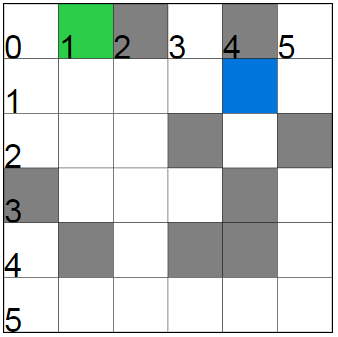
\includegraphics[width=0.20\textwidth]{image1}}
      & 
      \vspace{0.01cm}
      Schreibt Startpunkt in bekannte Liste mit Distanzwert.
      & 
      \vspace{0.01cm}
      $(4/1)\ d = 4$
      & 
      \vspace{0.01cm}
      --
      \\ \bottomrule %%%%%%%%%%%%%%%%%%%%%%%%%%%%%%%%%%%%%%%%
      \raisebox{-\totalheight}{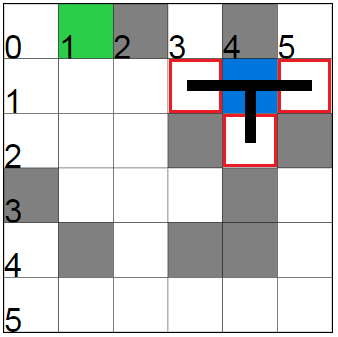
\includegraphics[width=0.20\textwidth]{image2}}
      & 
      \vspace{0.01cm}
      Berechne Distanzwert aller Nachbaren (rot markiert) und schreibe diese in die bekannte Knoten-Liste. Zeige auf den Vorgängigen Knoten (schwarzer Balken). Da $(4/1)$ alle bekannte Nachbaren hat, wird dieser Knoten in die Knoten-Liste der Untersuchten verschoben. Der Knopf mit den tiefsten $d$-Wert wird Angeschaut und der Prozess wird wiederholt.
      & 
      \vspace{0.01cm}
      $(3/1)\ d = 3$
      $(5/1)\ d = 5$
      $(4/2)\ d = 5$
      & 
      \vspace{0.01cm}
      $(4/1)\ d = 4$
      \\ \bottomrule %%%%%%%%%%%%%%%%%%%%%%%%%%%%%%%%%%%%%%%%
      \raisebox{-\totalheight}{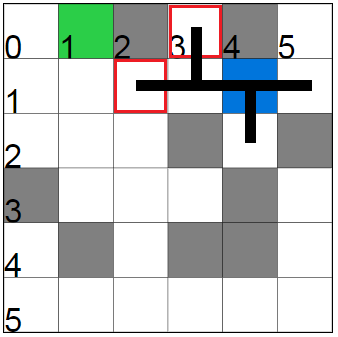
\includegraphics[width=0.20\textwidth]{image3}}
      & 
      \vspace{0.01cm}
      Da der Graph(3/1) Alle bekannten Nachbarn hat, wird dieser Knoten in der untersuchten Knoten-Liste verschoben.
      & 
      \vspace{0.01cm}
      $(3/0)\ d = 2$
      $(2/1)\ d = 2$
      $(5/1)\ d = 5$
      $(4/2)\ d = 5$
      & 
      \vspace{0.01cm}
      $(3/1)\ d = 3$
      $(4/1)\ d = 4$
      \\ \bottomrule %%%%%%%%%%%%%%%%%%%%%%%%%%%%%%%%%%%%%%%%
      \raisebox{-\totalheight}{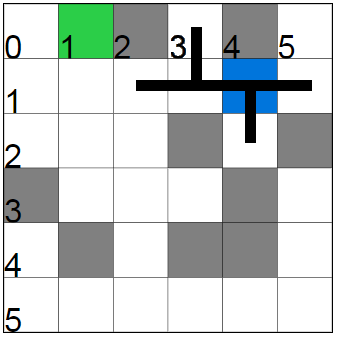
\includegraphics[width=0.20\textwidth]{image4}}
      & 
      \vspace{0.01cm}
      Falls Graph $(3/0)$ vor dem Graph $(2/1)$ angeschaut wird (gleiche $d$-Werte), wird dieser, da er keine gültigen Nachbaren hat, in die untersuchten Knoten-Liste geschrieben.
      & 
      \vspace{0.01cm}
      $(2/1)\ d = 2$
      $(5/1)\ d = 5$
      $(4/2)\ d = 5$
      & 
      \vspace{0.01cm}
      $(3/0)\ d = 2$
      $(3/1)\ d = 3$
      $(4/1)\ d = 4$
      \\ \bottomrule %%%%%%%%%%%%%%%%%%%%%%%%%%%%%%%%%%%%%%%%
      \raisebox{-\totalheight}{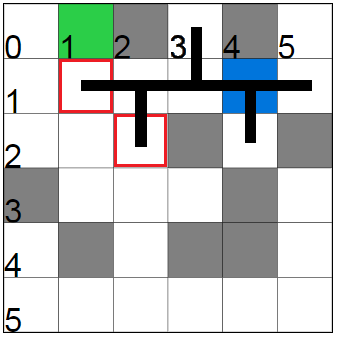
\includegraphics[width=0.20\textwidth]{image5}}
      & 
      \vspace{0.01cm}
      Der Prozess wird weitergeführt. Die Listen werden kontinuierlich aktualisiert.
      & 
      \vspace{0.01cm}
      $(1/1)\ d = 1$
      $(2/2)\ d = 2$
      $(3/1)\ d = 3$
      $(5/1)\ d = 5$
      $(4/2)\ d = 5$
      & 
      \vspace{0.01cm}
      $(3/0)\ d = 2$
      $(2/1)\ d = 2$
      $(4/1)\ d = 4$
      \\ \bottomrule %%%%%%%%%%%%%%%%%%%%%%%%%%%%%%%%%%%%%%%%
      \raisebox{-\totalheight}{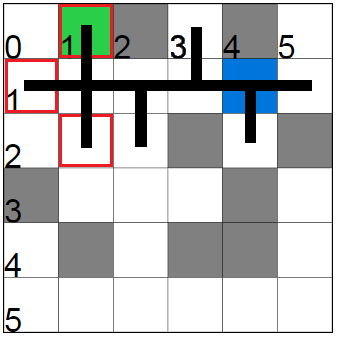
\includegraphics[width=0.20\textwidth]{image6}}
      & 
      \vspace{0.01cm}
      Der A* hat das Ziel erreicht und muss noch den einzelnen Graphen zurückfolgen bis zum Start und kennt somit den Weg.
      & 
      \vspace{0.01cm}
      $(1/0)\ d = 0$
      $(0/1)\ d = 2$
      $(1/2)\ d = 2$
      $(2/2)\ d = 2$
      $(3/1)\ d = 3$
      $(5/1)\ d = 5$
      $(4/2)\ d = 5$
      & 
      \vspace{0.01cm}
      $(1/1)\ d = 1$
      $(3/0)\ d = 2$
      $(2/1)\ d = 2$
      $(4/1)\ d = 4$
      \\ \bottomrule %%%%%%%%%%%%%%%%%%%%%%%%%%%%%%%%%%%%%%%%
    \end{tabular}
  \end{center}
\end{table}
\begin{table}[H]
  \begin{center}
    \begin{tabular}{ c  p{7cm}  p{2cm}   p{2cm} }
      \toprule
      \raisebox{-\totalheight}{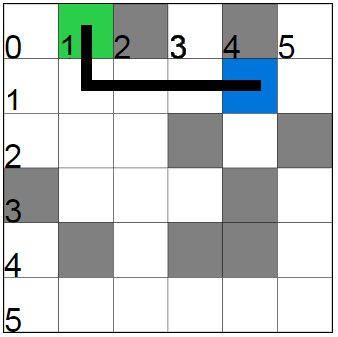
\includegraphics[width=0.20\textwidth]{image7}}
      & 
      \vspace{0.01cm}
      Die Suche ist Beendet.
      & 
      \vspace{0.01cm}
      --
      & 
      \vspace{0.01cm}
      --
      \\ \bottomrule %%%%%%%%%%%%%%%%%%%%%%%%%%%%%%%%%%%%%%%%
    \end{tabular}
  \end{center}
\end{table}



\subsection{BestFirstFinder}

Wie der Name schon sagt sucht dieser Pathfind-Algorithmus nach dem
erstbesten Weg zum Ziel. Im Vergleich zum A-Star hat dieser bloss eine
Liste mit offenen Knoten. Mit der Manhattan Heuristik wird nur der Weg
zum tiefsten Distanz wert Graph in diese Liste eingetragen, somit schaut
der Bestfirstfinder nicht auf alle nachbarknoten.

\subsubsection{Funktionsweise}

Es wird eine Liste für die Offenen Knoten eröffnet und der Startknoten
wird eingetragen. Auch hier verweist jeder Knoten auf seinen Vorgänger.
Der beste Knoten aus der Liste wird n genannt. Schau die Nachbarn von n
an und bewerte diese mit der Heuristik, der beste Wert wird in die Liste
eingetragen und der Ablauf wird wiederholt. Kommt ein Knoten, der
angeschaut wird, nicht weiter, wird der zweitbeste Graph in der Liste
Angeschaut. Es kann einer weiten Liste hinzugefügt werden, die
geschlossene Liste, die den Lösungsweg direkt mit Abspeichert und
verhindert, dass dieser Algorithmus nicht in einer Endlosschleife endet.
\cite[Roblox Developer, 2018]{robdevbff}

\subsubsection{Beispiel}

Der Startpunkt ist blau und der Zielpunkt grün, wobei diagonale Verbindungen nicht verfügbar sind.

\begin{table}[H]
  \begin{center}
    \begin{tabular}{ c  p{9cm}   p{2cm}   p{1cm}}
      \toprule
      Bild & Ausführung & Liste \\ 
      \cmidrule(r){1-1}\cmidrule(lr){2-2}\cmidrule(l){3-3}
      \raisebox{-\totalheight}{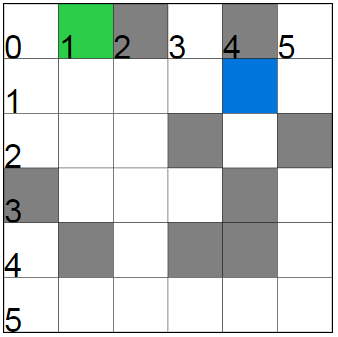
\includegraphics[width=0.20\textwidth]{image8}}
      & 
      \vspace{0.01cm}
      Schreibe Startpunkt in die Liste.
      & 
      \vspace{0.01cm}
      $(4/1)\ d = 4$
      \\ \bottomrule %%%%%%%%%%%%%%%%%%%%%%%%%%%%%%%%%%%%%%%%
      \raisebox{-\totalheight}{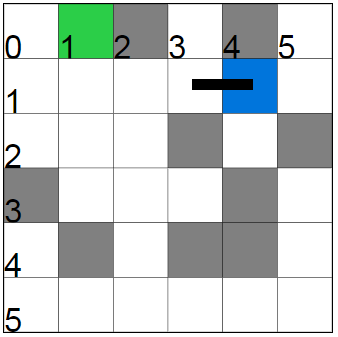
\includegraphics[width=0.20\textwidth]{image9}}
      & 
      \vspace{0.01cm}
      Wähle den besten Nachbar, anhand seiner Distanz Wert d, hier ist es Graph $(3/1)$. Schreibe diesen Wert in die Liste.
      & 
      \vspace{0.01cm}
      $(3/1)\ d = 3$
      $(4/1)\ d = 4$
      \\ \bottomrule %%%%%%%%%%%%%%%%%%%%%%%%%%%%%%%%%%%%%%%%
      \raisebox{-\totalheight}{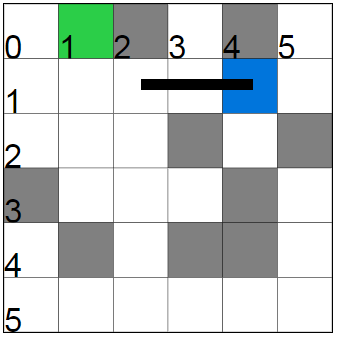
\includegraphics[width=0.20\textwidth]{image10}}
      & 
      \vspace{0.01cm}
      Wiederhole die Ausführung bis das Ziel erreicht wurde.
      & 
      \vspace{0.01cm}
      $(2/1)\ d = 2$
      $(3/1)\ d = 3$
      $(4/1)\ d = 4$
     \\ \bottomrule %%%%%%%%%%%%%%%%%%%%%%%%%%%%%%%%%%%%%%%%
      \raisebox{-\totalheight}{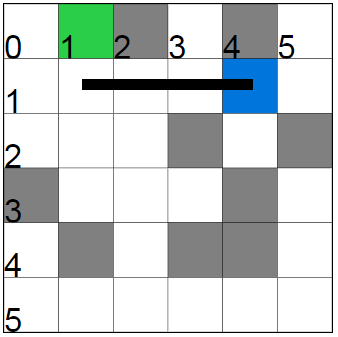
\includegraphics[width=0.20\textwidth]{image11}}
      & 
      \vspace{0.01cm}
      --
      & 
      \vspace{0.01cm}
      $(1/1)\ d = 1$
      $(2/1)\ d = 2$
      $(3/1)\ d = 3$
      $(4/1)\ d = 4$
     \\ \bottomrule %%%%%%%%%%%%%%%%%%%%%%%%%%%%%%%%%%%%%%%%
      \raisebox{-\totalheight}{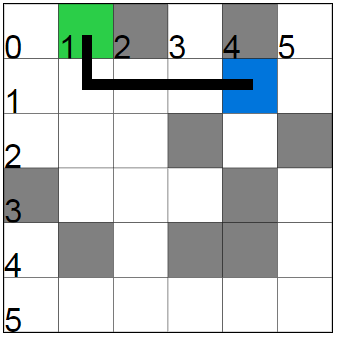
\includegraphics[width=0.20\textwidth]{image12}}
      & 
      \vspace{0.01cm}
      Der Weg wurde gefunden.
      & 
      \vspace{0.01cm}
      $(1/0)\ d = 0$
      $(1/1)\ d = 1$
      $(2/1)\ d = 2$
      $(3/1)\ d = 3$
      $(4/1)\ d = 4$
     \\ \bottomrule %%%%%%%%%%%%%%%%%%%%%%%%%%%%%%%%%%%%%%%%
    \end{tabular}
  \end{center}
\end{table}

\subsection{BreadthFirstFinder}

Der BreadthFirstFinder benutzt keine Heuristik, da er sein Weg über die
Breitensuche findet. Er Expandiert in jede Richtung gleich schnell und
bewegt sich nicht wie die anderen zwei Pathfinder in Richtung Ziel. Wenn
alle Knoten mit der gleichen Distanz zum Start angeschaut sind, beginnt
er mit der Suche der eins weiter entfernten Knoten. Dieser Pathfinder
besitzt eine Liste in der er die noch zu bearbeitenden Knoten speichert,
beginnend mit dem am Start nächsten Knoten.
\cite[Brilliant.org]{brilliantbfs}

\subsubsection{Funktionsweise}

Beginne beim Startpunkt und Speichere ihn in die Warteliste. Schaue am
obersten Knoten in der Warteschlange dessen Nachbarn an und prüfe ob
eines der Ausgewählten Knoten der Zielknoten ist. Ist dies der Fall wird
die Suche Abgebrochen, da der Weg Gefunden wurde. Falls keiner der
Knoten der Zielknoten ist, speichere die neuen Knoten in die Warteliste
an Hinterste Stelle und entferne den Ausgewählten Knoten. Jeder Knote
der neu gefunden wird zeigt auf den ausgewählten Knoten.

\subsubsection{Beispiel}

Der Startpunkt ist blau und der Zielpunkt grün. Diagonale Verbindungen sind nicht verfügbar.

\begin{table}[H]
  \begin{center}
    \begin{tabular}{ c  p{9cm}   p{2cm}   p{1cm}}
      \toprule
      Bild & Ausführung & Liste \\ 
      \cmidrule(r){1-1}\cmidrule(lr){2-2}\cmidrule(l){3-3}
      \raisebox{-\totalheight}{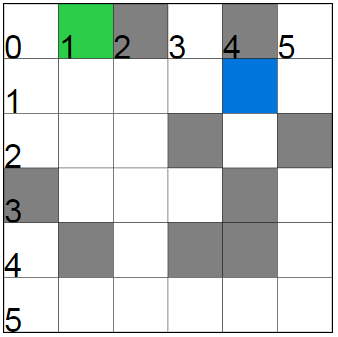
\includegraphics[width=0.20\textwidth]{image13}}
      & 
      \vspace{0.01cm}
      Schreibe den Startpunkt in die Liste.
      & 
      \vspace{0.01cm}
      $(4/1)$
     \\ \bottomrule %%%%%%%%%%%%%%%%%%%%%%%%%%%%%%%%%%%%%%%%
      \raisebox{-\totalheight}{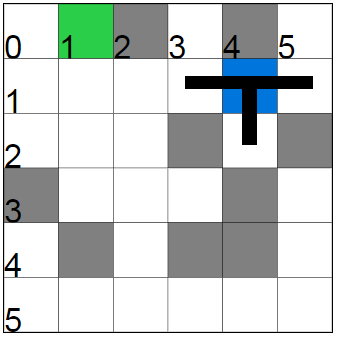
\includegraphics[width=0.20\textwidth]{image14}}
      & 
      \vspace{0.01cm}
      Schaue alle Nachbarn an und speichere diese in die Liste an hinterste Stelle. Falls keiner der neuen Knoten das Ziel ist, führe suche fort. Jeder neue Graph verweist auf den Vorgänger. Entferne aktuellen ausgewählten Knoten $(4/1)$.
      & 
      \vspace{0.01cm}
      $(3/1)\ \ $
      $(5/1)\ \ $
      $(2/1)\ \ $
     \\ \bottomrule %%%%%%%%%%%%%%%%%%%%%%%%%%%%%%%%%%%%%%%%
      \raisebox{-\totalheight}{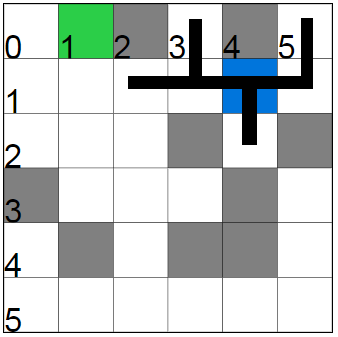
\includegraphics[width=0.20\textwidth]{image15}}
      & 
      \vspace{0.01cm}
      Schaue alle Nachbarn der zurzeit in der Liste stehenden Knoten und Wiederhole alles vom oben genannte. 
      & 
      \vspace{0.01cm}
      $(3/1)\ \ $
      $(2/1)\ \ $
      $(5/1)\ \ $
     \\ \bottomrule %%%%%%%%%%%%%%%%%%%%%%%%%%%%%%%%%%%%%%%%
      \raisebox{-\totalheight}{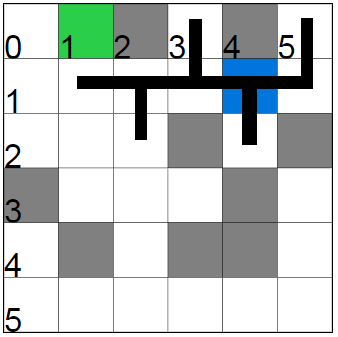
\includegraphics[width=0.20\textwidth]{image16}}
      & 
      \vspace{0.01cm}
      --
      & 
      \vspace{0.01cm}
      $(1/1)\ \ $
      $(2/2)\ \ $
     \\ \bottomrule %%%%%%%%%%%%%%%%%%%%%%%%%%%%%%%%%%%%%%%%
      \raisebox{-\totalheight}{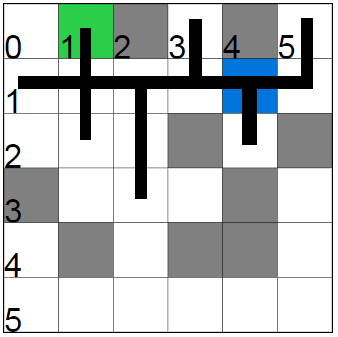
\includegraphics[width=0.20\textwidth]{image17}}
      & 
      \vspace{0.01cm}
      Das Ziel Wurde Gefunden und die Suche kann beendet werden. Folgen vom Ziel zum Start und gib den Lösungsweg aus.
      & 
      \vspace{0.01cm}
      $(0/1)\ \ $
      $(1/0)\ \ $
      $(1/2)\ \ $
      $(2/3)\ \ $
     \\ \bottomrule %%%%%%%%%%%%%%%%%%%%%%%%%%%%%%%%%%%%%%%%
      \raisebox{-\totalheight}{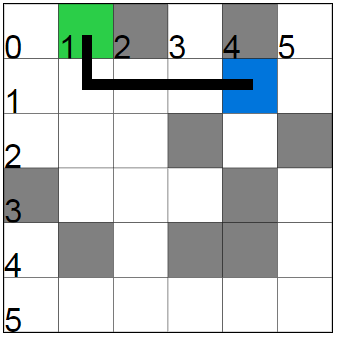
\includegraphics[width=0.20\textwidth]{image12}}
      & 
      \vspace{0.01cm}
      Der Weg wurde gefunden.
      & 
      \vspace{0.01cm}
      --
     \\ \bottomrule %%%%%%%%%%%%%%%%%%%%%%%%%%%%%%%%%%%%%%%%
    \end{tabular}
  \end{center}
\end{table}

\section{Vor- und Nachteile der einzelnen Pathfinder}

Anhand der Beispiele am gleichen Raster sieht man sehr gut, dass alle
drei Pathfinder den gleichen Weg finden durch unterschiedliche Methoden.

Der A-Star führt viele Heuristik Berechnungen durch, da er von jedem
Knoten die Distanz zum Ziel speichern möchte. Dies erfordert mehr
Rechenleistung beziehungsweise mehr Operationen als die beiden anderen.
Bei Komplexeren Raste wird er jedoch immer den besseren Weg finden.

Der BestFirstFinder untersucht nur den zuerst gefunden besten Weg und
sucht daher zuerst in der tiefe. Er braucht weniger Rechenleistung als
der A-Star, kann aber mühe bekommen, falls der erst gesuchte Weg in eine
Sackgasse führt. In diesem Beispiel musste er weniger Knoten anschauen
als der A-Star, obwohl er die gleiche Heuristik benutzt.

Der BreadthFirstFinder suche alle ihm am nächsten gelegenen Knoten ab
und wird immer auf eine Lösung kommen auf Kosten der ``unnötigen''
Knoten die weiter entfernt zum Ziel als seine aktuelle Position. Die
Warteliste wird mit jeder neuen Expansion um ein vielfaches grösser und
die Expansion Erweiterung wird über die Dauer langsamer.
